% CS 455, SP'22 Software Design Document template
% Software design template based on the template from
% https://tex.stackexchange.com/questions/42602/software-requirements-specification-with-latex
%
\documentclass[letterpaper,12pt,oneside,listof=totoc]{scrreprt}
\usepackage{listings}
\usepackage{graphicx}
\usepackage{underscore}
\usepackage{longtable}
\usepackage{comment}
\usepackage[bookmarks=true]{hyperref}
\hypersetup{
    bookmarks=false,                                % show bookmarks bar
    pdftitle={Software Design Document}, % title
%    pdfauthor={Yiannis Lazarides},                  % author
%    pdfsubject={TeX and LaTeX},                     % subject of the document
%    pdfkeywords={TeX, LaTeX, graphics, images},     % list of keywords
    colorlinks=true,                                % false: boxed links; true: colored links
    linkcolor=blue,                                 % color of internal links
    citecolor=black,                                % color of links to bibliography
    filecolor=black,                                % color of file links
    urlcolor=purple,                                % color of external links
    linktoc=page                                    % only page is linked
}%
\def\myversion{1.0 }

\date{\today}
\author{} % suppress warning, do not fill this in
\begin{document}

% we don't use \maketitle because we overide the default title page here
\begin{titlepage}
\flushright
\rule{\textwidth}{5pt}\vskip1cm
\Huge{SOFTWARE DESIGN DOCUMENT}\\
\vspace{1.5cm}
for\\
\vspace{1.5cm}
Data Storage System for Monitoring System\\
\vspace{1.5cm}
\LARGE{Release 1.0\\}
\vspace{1.5cm}
\LARGE{Version \myversion unapproved\\}
\vspace{1.5cm}
Prepared by Baxter Halder, Claire Hall, Kayla Jamar, Jennifer Olszyna\\
\vfill
\rule{\textwidth}{5pt}
\end{titlepage}

\tableofcontents
% this will be automatically created from chapters, sections, and subsections

\listoffigures
% this will be automatically created from the figure environment

\listoftables
% this will be automatically created from the table environment

\chapter*{Revision History}
% Update this table for each revision of the requirements
% Add the new content followed by a \hline

\begin{tabular}{| c | p{0.60\textwidth} | p{0.30\textwidth} |}
\hline
Date     & Description   & Revised by \\
\hline
03/11/22 & Initial draft & Data Store \\
\hline
03/16/22 & Notes & Data Store \\
\hline
03/20/22 & Additions & Data Store \\
\hline
\end{tabular}

% What is a Software Design Document (SDD)?
%
% Software design is a process by which the software requirements are translated into a representation of software components, interfaces, and data necessary for the implementation phase. The SDD shows how the software system will be structured to satisfy the requirements. It is the primary reference for code development and, therefore, it must contain all the information required by a programmer to write code. The SDD is typically performed in two stages. The first is a preliminary design in which the overall system architecture and data architecture is defined. In the second stage -- i.e., the detailed design stage -- more detailed data structures are defined and algorithms are developed for the defined architecture.
%
% This template is an annotated outline for a software design document adapted from the IEEE Recommended Practice for Software Design Descriptions. The IEEE Recommended Practice for Software Design Descriptions have been reduced in order to simplify this assignment while still retaining the main components and providing a general idea.
%

%----------------------------------------------------------------------------------------------------
\chapter{INTRODUCTION}

\section{Purpose}

This software design document describes the architecture and system design of CS455 Monitor System. This document will illustrate the purpose and complete declaration for the development of this system as well as explain the system’s  constraints, interface, and interactions with other external applications. This document is primarily intended to be proposed to a customer for his approval and act as a reference for developing the first version of the system for the development team.
\section{Scope}

The CS455 Monitor System software will monitor both the activity and health of all machines on a network. The system itself will be a combination of four sub-systems; Agents, a Monitoring Engine, a Data Store, and a Dashboard. The Engine and Data Store are hosted on the CS server. However, the Engine and Data Store will be portable to other server machines that run on a Unix-like OS. The Agents, installed on devices on the network, can run on both Windows and Unix-like systems. The Dashboard will display the status of the monitored machines. The Dashboard can be used on Windows or Ubuntu machines. Users will be able to view specific information such as CPU usage, memory usage, disk usage, and network usage of the monitored machines on the network from the Dashboard. This information passes through the Monitoring Engine to be validated, such as checking valid ranges for data, before being stored in the Data Store for the Dashboard to retrieve. Users will be able to view the specific machines the Agents are monitoring that are connected to the network in order to track down the cause of issues. Examples of these issues include a monitored machine being disconnected or unresponsive, a monitored machine's disk is close to or over capacity, a monitored machine's CPU usage is maxed out, which services should be running on the monitored machine that are not currently running, the network usage is less than the user expected for a monitored machine, or the monitored machine's memory usage is close to capacity. 


\section{Overview}

The database acts as a place to store collected metrics and logs. The database will be scalable to accommodate up to hundreds of active servers and a dozen active dashboards.The database system will be hosted on the CS server. The data storage will take data from the monitoring system and sort it into one of two fundamental types of data, metrics or logs. Metrics are numerical values that describe some aspect of a system at a particular point in time. They are lightweight and capable of supporting near real-time scenarios. Logs contain different kinds of data organized into records with different sets of properties for each type.
\section{References}

\begin{longtable}{ p{0.25\textwidth} p{0.60\textwidth} } 
   \textbf{ Standard} & \textbf{Reference }\\
    \hline
    SEI CERT & \href{https://wiki.sei.cmu.edu/confluence/display/seccode}{SEI CERT Secure Coding Practices}\\
    \hline
    Microsoft SDL & \href{https://www.microsoft.com/en-us/securityengineering/sdl/practices}{Microsoft SDL Secure Development Practices}\\
    \hline   
    SQL and PL/SQL Coding Standards  & \href{http://www.dba-oracle.com/t_plsql_best_practices_standards.htm}{PL/SQL best practice Standards tips}\\
    \hline
    Standard SQL Naming Conventions & \href{http://www.dba-oracle.com/standards_schema_object_names.htm}{Oracle naming standards tips}\\
    \hline
    JSON &  \href{https://datatracker.ietf.org/doc/html/rfc8259}{RFC 8259}\\
    \hline    
\caption{References}
\end{longtable}

\section{Definitions and Acronyms}

\begin{longtable}{| p{0.25\textwidth} | p{0.65\textwidth} |} 
    \hline
   \textbf{ Acronym or Abbreviation} & \textbf{Definition}\\
    \hline
    KPI & Key Performance Indicators are quantifiable measure of performance over time for a specific objective that provides the admin insights into the network. \\
    \hline
    QA & Quality assurance is a system for evaluating performance. \\
    \hline
    GUI & Graphical User Interface\\
    \hline
    SRS & Software Requirements Specifications\\
    \hline
    UNA & University of North Alabama\\
    \hline
    CS455 & The computer science class at the University of North Alabama in which this project is being made\\
    \hline
\caption{Acronyms and Abbreviations}
\end{longtable}


%----------------------------------------------------------------------------------------------------
\chapter{SYSTEM OVERVIEW}
%Give a general description of the functionality, context, and design of your project. Provide any background information if necessary.
% diagram
%big picture goal of software

The CS455 Monitor System is a network monitoring system that will monitor UNA's CS network in order to help users identify and address potential network problems as they occur. The system will automatically collect and store data, as well as provide warnings and error messages when certain events trigger, such as an unresponsive agent or disk is at capacity. However, the system will rely on users to see the messages and act on them; the system is \textbf{not} automated to handle the events. (As a specific example, if an error message pertaining to an unresponsive agent appears, it is the user's job to determine why the connection has failed and handle the issue.) The Monitor System contains four sub-systems working in tandem as shown in Figure~\ref{systemdiagram}; Agents, Monitoring Engine, Data Store, and a Dashboard.

\begin{figure}[h!]
\centering
\includegraphics[scale=0.35]{Data Store Folder/system_graph.png}
\caption{Database Design Depicted as an E/R Diagram}
\label{systemdiagram}
\end{figure}

The monitoring system is relatively simple conceptually. Agents, installed on devices connected to the network, will collect basic usage statistics such as CPU usage, memory usage, disk usage, network usage, and service applications that are currently running on the device. The frequency at which to collect data will be specified in the configuration text file (though in cases where a time is not specified there is a default time). The configuration file will also associate each agent with a unique ID and name corresponding to the device it is installed on in order to keep track of the data associated as it transfers through the system as a whole. This configuration file also contains the host name of the Engine should the user decide to port the Engine to another device. Each agent will automatically send its collected data to the Monitoring Engine over the network to be stored in the Data Store.

The Monitoring Engine (or simply the Engine), hosted on the CS server, will take in data from the Agents, perform sanity checks on the data, and then pass it on to the Data Store for storage. A "sanity check" is ensuring that incoming data is in a logical range. For instance, it is impossible for CPU usage to be above 100\%. It is impossible for the disk usage to be above 120\%. It is impossible for memory usage to be a negative percent. Should the Engine receive invalid data such as this, it will log an error to the Data Store. The Engine also contains a configuration file that details the host name of the Data Store that can be changed should the user want to port the Data Store to another device. This configuration file also knows the frequency it should be getting updates from each Agent. If the Engine receives no update from an Agent after that configured time frame, it logs an error message to the Data Store. The user will never interact directly with the Engine.

The Data Store, also hosted on the CS server, will take data from the Monitoring Engine and sort it into one of two fundamental types of data, metrics or logs. Metrics are numerical values that describe some aspect of a system at a particular point in time. Logs contain different kinds of data organized into records with different sets of properties for each type. The user will never directly interact with the Data Store. The Data Store acts solely as a place to store collected metrics and logs. The Data Store will be scalable to store information of up to fifty active Agents, process queries from up to a dozen active Dashboards, and be able retain data for up to a year. Users are able to remove or archive specific data in the Data Store.

The Dashboard will provide easy access to viewing the metrics of multiple different devices. Users will be able to view both current and past metrics for a device as well as see if there are connection issues with an Agent's monitored device. 

%----------------------------------------------------------------------------------------------------
\chapter{SYSTEM ARCHITECTURE}

\section{Architectural Design}
%big picture modules; high level subsystems. role and responsibilities.focus on data store
%Develop a modular program structure and explain the relationships between the modules to achieve the complete functionality of the system. This is a high level overview of how responsibilities of the system are partitioned and then assigned to subsystems. Identify each high level subsystem and the roles or responsibilities assigned to it. Describe how these subsystems collaborate with each other in order to achieve the desired functionality. Don't go into too much detail about the individual subsystems. The main purpose is to gain a general understanding of how and why the system was decomposed, and how the individual parts work together. Provide a diagram showing the major subsystems and data repositories and their interconnections. Refer to and describe the diagram in the narrative.
The Data Store, hosted on the CS server, will accept data sent from the Monitoring Engine and then store it for the user to access through the dashboard interface. 
The Date Store is composed of three majors components, a part to listen to the Engine, the database, and a part to listen to the Dashboard. As these components flow together and overlap heavily, they were not given individual identifying names. 


\section{Decomposition Description}
%UML with classes
%Provide a decomposition of each one of the subsystems in the architectural design. You may choose to give a functional description or an object oriented (OO) description. For a functional description use appropriate diagrams such as top-level data flow diagrams (DFD) and structured decomposition diagrams. For an OO description use the appropriate diagrams such as subsystem model, object diagrams, generalization diagram(s), aggregation diagram(s), interface, and specification diagrams.
The first component listens to the Engine and then receives either error messages or JSON files containing information from the Agents. 

The second component is the database itself that will implemented as a MariaDB database hosted on the CS server. The database's schema is depicted in Figure~\ref{erdiagram} as an E/R diagram.
It is assumed by the Data Store that the data is valid, so once the file is received the Data Store will parse out the information contained in the file and insert it into the \textit{devices} entity or parse and insert the error message details into the \textit{error_log} entity. A database entity is a thing, person, place, unit, object or any element data should be stored in the form of properties. The Data Store's database will be comprised of two entities. \textit{devices}, and the \textit{error_log}. Each entry in the \textit{devices} entity represents a device with an Agent installed on it. 

The last component is the part listening to the Dashboard for either queries or error messages. Error messages are processed the same way ones from the Engine are, and quires are transforms into SQL quires and processed. The Data Store then returns the requested data to the Dashboard.

\begin{figure}[h!]
\centering
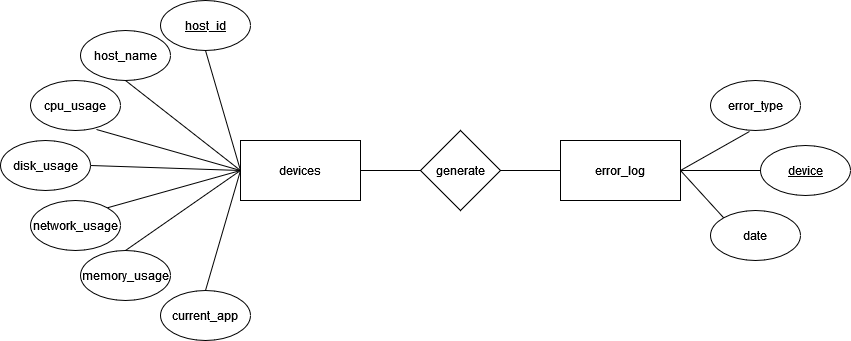
\includegraphics[scale=0.45]{Data Store Folder/er_diagram.png}
\caption{Database Design Depicted as an E/R Diagram}
\label{erdiagram}
\end{figure}

\section{Design Rationale}
%justify why you chose the library and why you chose over another lib
%Discuss the rationale for selecting the architecture described in the previous section including critical issues and trade/offs that were considered. You may discuss other architectures that were considered, provided that you explain why you didn't choose them.
MariaDB was chosen over SQL or MySQL due to the team's familiarly with the database type as well as the numerous JSON functions built into it.

%----------------------------------------------------------------------------------------------------
\chapter{DATA DESIGN}

\section{Data Description}
%Explain how the information domain of your system is transformed into data structures. Describe how the major data or system entities are stored, processed and organized.
%how data is moving through system
The Data Store receives data from the Engine in the form of a JSON file. This information will be passed to a memory buffer where a function will parse out the information in the file. This information will be inserted into the \textit{devices} entity and continuously updated as the Engine sends updated files. On the - figuratively speaking- other end the Data Store will receive queries from the Dashboard and then send back the results.

\section{Data Dictionary}
%Alphabetically list the system entities or major data along with their types and descriptions. If you provided a functional description in the ``Decomposition'' Section, list all the functions and function parameters. If you provided an OO description, list the objects and the associated attributes, methods and method parameters.
The Data Store will receive a JSON object in the form of a text file. The Data Store will transform the file into a SQL insert statement and insert it into the \textit{devices} entity. 

%----------------------------------------------------------------------------------------------------
\chapter{COMPONENT DESIGN}
%can use sort algorithm with reference
% instructions for devs; pseudocode allowed

MariaDB SQL queries\\

Receive message and store messages\\

Create device table with entities of host ID, host name, CPU usage, disk usage, network usage, memory usage\\

JSON_EXTRACT() function used to parse data from the JSON document 

Insert host ID

Insert host name

Insert CPU usage

Insert disk usage

Insert network usage 

Insert memory usage\\


Create error log table with entities of error type, device, and date

Insert error type 

Insert device 

Insert date\\




Constraint used to validate request 

Send data to dashboard 


%Give a detailed description of what each component does in a systematic way. If you gave a functional description in ``Decomposition'' section, provide a summary of your algorithm for each function using either a procedural description language (PDL) or pseudocode. If you gave an OO description, summarize each object's member functions for all the objects listed using PDL or pseudocode. Describe any local data when necessary. This section should include enough information for a competent programmer to implement each component. It should NOT be actual code.




%----------------------------------------------------------------------------------------------------
\chapter{HUMAN INTERFACE DESIGN}
% 6.1 & 6.2
% have way to start and end, if issues starting up give message.
% "if starts up correctly you wont see anything, but if you have an issue you will see an % diagnostic message like so "


\section{Overview of User Interface}

%Describe the functionality of the system from the user's perspective. Explain how the user will be able to interact with the system to complete all the expected features and the feedback information that will be displayed for the user.

The Data Store creates database tables and inserts data into the tables upon receiving information from the Engine. If there are issues with receiving messages from the Engine, an error message will occur. The Data Store will access data that is stored in the database tables upon receiving a query from the Dashboard. If the query fails, an error message will occur. \\

\section{Screen Designs}

%Show mock-ups of the interface from the user's perspective. These can be hand drawn or you can use a software tool to create illustrations. Just make them as accurate as possible. Graph paper works well when hand drawing the screens.

Nothing will appear or be visible to the user if the Data Store successfully runs. If issues occur and the Data Store does not successfully run, a diagnostic message will occur. 


%----------------------------------------------------------------------------------------------------
\chapter{REQUIREMENTS MATRIX}
% table: list function and then ID from SRS of requirement that function fulfils
%Provide a cross-reference that traces each component and data structure to the requirement(s) in the SRS document. Use a tabular format to show which system components satisfy each one of the functional and non-functional requirements. Refer to the requirements by the number/code used in the SRS document.

The requirements matrix provides a cross-reference that traces each component and data structure to the requirements in the Software Requirements Specification document. See table ~\ref{Requirements Matrix}.

\begin{longtable}{ p{0.10\textwidth} |  p{0.25\textwidth} | p{0.50\textwidth} }
\hline
\textbf{ID} & \textbf{Requirement} & \textbf{System Component} \\
\hline
SR01 & Engine can create and send a network message to the Data Store & Database Tables Storing Received Messages\\
\hline
SR02 & Data store validates requests from Dashboard & Database Table Constraints\\
\hline
SR06 & Data Store sends data to the Dashboard & SQL Queries\\
\hline
SR11 & Engine sends an error message to the Data Store when upon receiving invalid data & Error Log Table Storing Error messages\\
\hline
SR13 & Users can view CPU usage & Device Table Storing CPU Usage, SQL Queries \\
\hline
SR14 & Users can view memory usage & Device Table Storing Memory Usage, SQL Queries\\
\hline
SR15 & Users can view disk usage & Device Table Storing Disk Usage, SQL Queries\\
\hline
SR16 & Users can view network usage & Device Table Storing Memory Network, Queries\\
\hline
SR17 & Users can view monitored services & Device Table Storing Monitored Service, SQL Queries\\
\hline
SR23 & Data Store runs on Unix-like & CS Server (cs.csis.work)\\
\hline
SR26 & Data Store is able to scale in size & Horizontal and Vertical Scaling\\
\hline
SR27 & Data store can hold data for at least a year & Analyze Table, Check Table, Optimize Table, Repair Table, and Get Rows Count Queries\\
\hline
SR28 & Data can be archived or removed by users & Archive Database Tables, Insert and Delete Queries\\
\hline
QR5 & Document and follow a coding style & SEI CERT\\
\hline
QR7 & System can be ported to other devices & Configuration File\\
\hline
\caption{Requirements Matrix}
\label{Requirements Matrix}
\end{longtable}

\end{document}
